\documentclass[main.tex]{subfiles}

\begin{document}

\chapter{Trigonometria e Vetores}

\section{Apresentação}

Além de ser uma disciplina em si mesma, a Geometria Analítica inaugura um jeito de encarar problemas geométricos que será o mais comum durante disciplinas matemáticas no ensino superior. A Geometria Analítica nasce da junção de técnicas da Álgebra (equações, funções) e da Geometria Plana (medidas, ângulos, semelhança) graças ao uso de um sistema de eixos cartesianos. Mas além de permitir o uso de elementos desses dois universos, essa junção abre portas para a criação de novos elementos, como os vetores.

O que faremos neste capítulo é revisitar alguns conceitos centrais da trigonometria que você deve ter estudado no Ensino Médio, mas agora enfatizaremos os usos que serão feitos na disciplina de Geometria Analítica. Além disso, utilizaremos constantemente eixos cartesianos em questões que poderiam ser formuladas apenas com elementos geométricos e utilizaremos vetores para formular e resolver algumas das questões.

\newpage

\section{Pré-requisitos e Auto-avaliação inicial}

Os pré-requisitos para este capítulo são:
\begin{itemize}
 \item Noções básicas de trigonometria no triângulo retângulo (seno e cosseno);
 \item Noções básicas sobre plano cartesiano (coordenadas).
\end{itemize}

Esses tópicos não serão cobertos durante as atividades de tutoria. Se você acha que não sabe o suficiente sobre algum deles, sugerimos que se procure material de apoio antes de começar a resolver as questões desse capítulo.

Antes de começar, indique o quanto você acha que sabe sobre os seguintes itens:

\begin{center}
 \begin{tabular}{|p{35mm}||p{15mm}|p{15mm}|p{15mm}|p{15mm}|} 
 \hline
   & Nada & Muito pouco & Noções gerais & Bastante\\
 \hline
 Calcular seno e cosseno em um triângulo retângulo &  &  &  &  \\ 
 \hline
 Obter um ângulo sabendo o seu seno ou cosseno &  &  &  &  \\
 \hline
 Usar seno e cosseno em uma calculadora &  &  &  &  \\
 \hline
 Representar vetores &  &  &  &  \\
 \hline
\end{tabular}
\end{center}

\newpage

\section{Questões diagnósticas}

\begin{diagnostico}
Considerando a figura abaixo, calcule:
\begin{enumerate}[a)]
  \item A medida do segmento $\overline{AB}$.
  \item Seja $D$ a intersecção do lado $CB$ com a altura do triângulo relativa ao vértice $A$, calcule o comprimento de $\overline{BD}$.
\end{enumerate}
\end{diagnostico}
 
\begin{figure}[h]
\centering
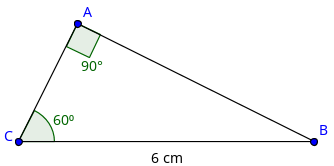
\includegraphics[width=0.4\textwidth]{./img/c4d1.png}
\end{figure}

\begin{diagnostico}
Qual é a medida em graus do ângulo formado entre o eixo $X$ e o segmento de reta que liga a origem ao ponto $(3;1)$? \textit{Você pode usar a calculadora se julgar necessário.}
\end{diagnostico}

\newpage

\section{Questões}

Lembre-se de checar com seu tutor em qual questão você deve começar.

\subsection*{Seno e cosseno}

Em Geometria Plana, definimos seno e cosseno de um ângulo $\alpha$ como sendo iguais a:

\begin{caixaExemplo}
$$ \sin(\alpha) = \frac{\text{cateto oposto}}{\text{hipotenusa}} \text{ e } \cos(\alpha) = \frac{\text{cateto adjacente}}{\text{hipotenusa}}$$
\end{caixaExemplo}

O valor do seno e do cosseno dos ângulos 0\degree, 30\degree, 45\degree, 60\degree e 90\degree, chamados de ângulos notáveis, são simples e recorrentes em problemas de geometria plana, portanto, espera-se que estudantes os tenham memorizados.

\begin{caixaExemplo}
\begin{center}
 \begin{tabular}{|c| c c c c c |} 
 \hline
  & 0\degree & 30\degree & 45\degree & 60\degree & 90\degree\\
 \hline
  seno & $0$ & $\frac{1}{2}$ & $\frac{\sqrt{2}}{2}$ & $\frac{\sqrt{3}}{2}$ & $1$\\ 
 \hline
 cosseno & $1$ & $\frac{\sqrt{3}}{2}$ & $\frac{\sqrt{2}}{2}$ & $\frac{1}{2}$ & $0$\\
 \hline
\end{tabular}
\end{center}
\end{caixaExemplo}

\begin{questao}
Sabendo que $\overline{AB}=6$ e $B \hat{C} D$ na figura abaixo, calcule o comprimento dos segmentos:
\begin{enumerate}[a)]
\item $\overline{BC}$
\item $\overline{BD}$
\item $\overline{AD}$
\end{enumerate}
\end{questao}

\begin{gabarito}
	\begin{gabaritoQuestao}
		a) $3$, b) $2\sqrt{3}$, c) $2\sqrt{3}$.
	\end{gabaritoQuestao}
\end{gabarito}

\begin{figure}[h]
\centering
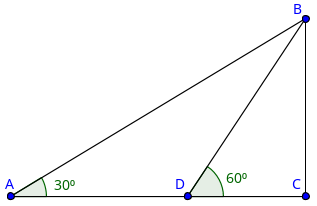
\includegraphics[width=0.5\textwidth]{./img/c4q1.png}
\end{figure}

\subsection*{Seno e cosseno de ângulos quaisquer}

Os valores listados na tabela acima são importantes, mas ângulos podem ocorrer em quaisquer medidas. Nesses casos, você pode usar a sua calculadora (a menos que o valor exato ou alguma aproximação específica seja fornecida). Na maioria dos celulares os botões cos e sin ficam disponíveis apenas no modo científico (acessível ao colocar o celular na horizontal) e é fundamental checar se o ângulo deve ser dado em graus (DEG) ou radianos (RAD).

\begin{questao}
Use o seu celular pra obter:
\begin{enumerate}[a)]
\item $\sin(\frac{4\pi}{9})$, arredondado para 2 casas decimais.
\item $\cos(\frac{\pi}{12})$, arredondado para 2 casas decimais.
\item $\sin(18\degree)$, arredondado para 1 casa decimal.
\item $\cos(22.5\degree)$, arredondado para 1 casa decimal.
\item $\cos(1,5)$, arredondado para 2 casas decimais.
\end{enumerate}
\end{questao}

\begin{gabarito}
	\begin{gabaritoQuestao}
		a) $0,98$, b) $0,97$, c) $0,3$, d)$0,9$, e) $0,07$.
	\end{gabaritoQuestao}
\end{gabarito}

Deste ponto em diante, use a calculadora sempre que os ângulos envolvidos não sejam notáveis e quando nenhuma aproximação for fornecida. Caso nenhum arredondamento específico seja pedido, use sempre duas casas decimais.

\subsection*{Geometria com ângulos quaisquer}

\begin{questao}
Sabendo que na figura abaixo $\overline{AC}=4$ obtenha a medida dos segmentos pedidos abaixo. Use uma calculadora se necessário.
\begin{enumerate}[a)]
\item A altura do triângulo relativa ao lado $\overline{AB}$.
\item $\overline{CB}$
\end{enumerate}
\end{questao}

\begin{gabarito}
	\begin{gabaritoQuestao}
		a) $3,76$, b) $9,24$.
	\end{gabaritoQuestao}
\end{gabarito}


\begin{figure}[h]
\centering
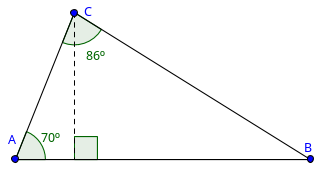
\includegraphics[width=0.5\textwidth]{./img/c4q3.png}
\end{figure}

\subsection*{Obtendo o ângulo a partir do seno ou cosseno}

Se você souber que um ângulo de um triângulo retângulo tem seno igual a $\frac{1}{2}$ você sabe que se trata de um ângulo de 30\degree, mas isso só é possível porque este valor está entre os poucos que fazem parte da tabela de valores notáveis. A pergunta então é como você pode saber a medida em graus ou radianos de um ângulo cujo seno é igual a $0,7$, por exemplo?

A resposta está nas funções \textbf{arcosseno} (arcsin, em inglês) e \textbf{arcocosseno} (arccos, em inglês). Por serem as funções inversas do seno e do cosseno, também são chamadas algumas vezes de $\sin^{-1}$ e $\cos^{-1}$. Tente encontrar essas funções na calculadora do seu celular (além de acessar o modo científico, em algumas calculadoras é necessário ativar o modo de funções inversas - INV) e calcular $\sin^{-1}(0.5)$. O resultado deve ser aproximadamente $0.5236$ (que é igual a $\pi/6$) ou $30\degree$.

\begin{questao}
Use as funções $\sin^{-1}$ e $\cos^{-1}$ da sua calculadora para obter:
\begin{enumerate}[a)]
\item A medida em radianos, com duas casas decimais, do ângulo cujo seno é igual a $0,7$. Dica: procure pela opção DEG e RAD na calculadora para alternar entre graus e radianos.
\item A medida em radianos, com duas casas decimais, do ângulo cujo cosseno é igual a $0,4$.
\item A medida em graus, com zero casas decimais, do ângulo cujo seno é igual a $0,6$. 
\item A medida em graus, com zero casas decimais, do ângulo cujo cosseno é igual a $0,87$.
\end{enumerate}
\end{questao}

\begin{gabarito}
	\begin{gabaritoQuestao}
		a) $0,78$, b) $1,16$, c) $37\degree$, d) $30\degree$.
	\end{gabaritoQuestao}
\end{gabarito}

\subsection*{Ângulos e eixos cartesianos}

\begin{questao}
Considerando a imagem abaixo, calcule:
\begin{enumerate}[a)]
\item O comprimento do segmento $\overline{OP}$. \textit{$O$ se refere à origem, ou seja, ao ponto $(0;0)$}.
\item O seno e o cosseno do ângulo determinado pelo segmento $\overline{OP}$ e o eixo $X$. 
\item A medida em radianos e em graus desse ângulo.
\end{enumerate}
\end{questao}

\begin{gabarito}
	\begin{gabaritoQuestao}
		a) $\sqrt{13}$, b) o seno vale $2\sqrt{13}/13$ e o cosseno $3\sqrt{13}/13$, c) $0,59$ e $34\degree$.
	\end{gabaritoQuestao}
\end{gabarito}

\begin{figure}[h]
\centering
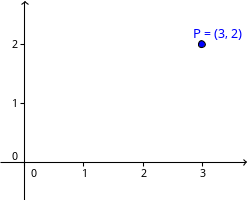
\includegraphics[width=0.5\textwidth]{./img/c4q5.png}
\end{figure}

\subsection*{Vetores}

Na questão anterior, mais do que o ponto $P$, o elemento chave foi o segmento $\overline{OP}$. Em Geometria Analítica um dos conceitos mais importantes é o de \textbf{vetor}. Um vetor pode ser pensado como um segmento com direção, tipicamente uma seta. No caso da questão anterior, poderíamos falar do vetor $\overrightarrow{OP}$, ou simplesmente $\overrightarrow{P}$ uma vez que a outra extremidade é a origem.

Todo vetor possui três propriedades que o definem: a \textbf{norma} (nome dado ao comprimento se estivéssemos pensando em um segmento), a \textbf{direção} (dada pelo ângulo entre o vetor e a parte positiva do eixo X no sentido anti-horário) e o \textbf{sentido} (no caso do nosso exemplo, o sentido é de $O$ a $P$ e não de $P$ a $O$).

Pode parecer artificial usar esse conceito já que ele pode ser descrito em termos dos pontos das extremidades do vetor ou do segmento conectando esses dois pontos, mas o conceito de vetor abre novas possibilidades bastante poderosas em matemática pura, que serão estudadas em disciplinas como Geometria Analítica e Álgebra Linear, e em diversas aplicações, em Física e engenharias em geral.

Não estudaremos essas potencialidades dos vetores neste capítulo, mas utilizaremos o conceito em algumas questões para que você se familiarize com ele gradualmente.

\begin{questao}
Considere os dois vetores representados abaixo.
\begin{enumerate}[a)]
\item Calcule a norma de $\overrightarrow{V}$ e $\overrightarrow{U}$.
\item Obtenha, em graus, os ângulos determinados por $\overrightarrow{V}$ e $\overrightarrow{U}$.
\item Determine, em graus, a medida do ângulo entre $\overrightarrow{V}$ e $\overrightarrow{U}$.
\end{enumerate}
\end{questao}

\begin{gabarito}
	\begin{gabaritoQuestao}
		a) $\Arrowvert V \Arrowvert = \sqrt{5}$ e $\Arrowvert U \Arrowvert = \sqrt{10}$, b) $63\degree$ e $18\degree$, c) $45\degree$.
	\end{gabaritoQuestao}
\end{gabarito}


\begin{figure}[h]
\centering
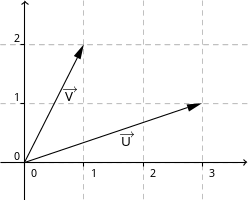
\includegraphics[width=0.5\textwidth]{./img/c4q6.png}
\end{figure}

\subsection*{Mais vetores}

\begin{questao}
Determine as coordenadas e represente em um plano cartesiano os vetores cuja norma e ângulo são dados abaixo.
\begin{enumerate}[a)]
\item Vetor $\overrightarrow{V}$ com norma $3$ e ângulo $40\degree$.
\item Vetor $\overrightarrow{U}$ com norma $2$ e ângulo $150\degree$.
\end{enumerate}
\end{questao}

\begin{gabarito}
	\begin{gabaritoQuestao}
		a) $(2,30;1,93)$, b) $(-\sqrt{3};1,00)$.
	\end{gabaritoQuestao}
\end{gabarito}

\subsection*{Área entre vetores}

\begin{questao}
Considere os dois vetores da questão 6 ($\overrightarrow{V}=(1,2)$ e $\overrightarrow{U}=(3,1)$). Vamos calcular a área do triângulo determinado pela origem e pela extremidade desses vetores.
\begin{enumerate}[a)]
\item Recupere da questão 6 os valores das normas e do ângulo entre os vetores e represente o triângulo em questão em um plano cartesiano com essas informações.
\item Trace a altura do triângulo relativa à $\overrightarrow{U}$.
\item Calcule o comprimento dessa altura usando o seno do ângulo entre os vetores.
\item Calcule a área do triângulo usando $\overrightarrow{U}$ como base.
\end{enumerate}
\end{questao}

\begin{gabarito}
	\begin{gabaritoQuestao}
		c) $\sqrt{10}/2$, d) $\frac{5}{2}$.
	\end{gabaritoQuestao}
\end{gabarito}

\begin{figure}[h]
\centering
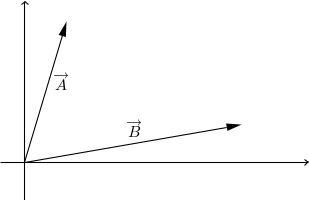
\includegraphics[width=0.6\textwidth]{./img/c4q8.png}
\end{figure}

Se não tivéssemos usado valores numéricos para essa questão, você teria chegado à fórmula $A=\frac{1}{2} \cdot \text{lado 1} \times \text{lado 2} \times \sin(\alpha)$, em que o comprimento dos lados são iguais a norma dos vetores e $\alpha$ é o ângulo entre eles.

Imagine agora que o comprimento dos dois vetores estão fixos, mas é possível girar $\overrightarrow{A}$ em torno da origem. A medida que $\overrightarrow{A}$ se aproxima de $\overrightarrow{B}$, três variáveis se comportam de maneira semelhante: o ângulo $\alpha$ entre os vetores, a área do triângulo determinado pelos vetores e $\sin(\alpha)$ diminuem. Por outro lado, se afastarmos $\overrightarrow{A}$ de $\overrightarrow{B}$ até formar um ângulo reto essas três variáveis aumentam.

De certa maneira podemos interpretar essas três variáveis como sendo medidas de perpendicularidade entre dois vetores. Em Geometria Analítica essa ideia será capturada pela operação chamada \textbf{produto vetorial}.

\subsection*{Área entre vetores, 2}

\begin{questao}
Calcule a área do triângulo determinado pelos vetores $\overrightarrow{V}=(2;2)$ e $\overrightarrow{U}=(4;1)$ usando a estratégia usada na questão anterior.
\end{questao}

\begin{gabarito}
	\begin{gabaritoQuestao}
		a) $2,42$.
	\end{gabaritoQuestao}
\end{gabarito}

Note que o valor obtido foi muito próximo de 3. Na realidade, se os cálculos fossem realizados sem aproximações, o resultado seria exatamente 3 e isso poderia ser verificado pelo método de ``contar quadradinhos'' já que as coordenadas dos vetores são números inteiros (bastaria considerar a área do retângulo $4 \times 2$ construído ao redor do triângulo e subtrair a área dos triângulos que não interessam. Tente!).

\subsection*{Projeção ortogonal}

\begin{questao}
Considere os dois vetores da questão anterior ($\overrightarrow{V}=(2,2)$ e $\overrightarrow{U}=(4,1)$).
\begin{enumerate}[a)]
\item Recupere da questão anterior os valores das normas e do ângulo entre os vetores e represente-os em um plano cartesiano.
\item Trace a altura do triângulo relativa à $\overrightarrow{U}$ e chame de $C$ a intersecção dessa altura com $\overrightarrow{U}$.
\item Calcule o comprimento do vetor $\overrightarrow{OC}$.
\end{enumerate}
\end{questao}

\begin{gabarito}
	\begin{gabaritoQuestao}
		a) $2.301$, b) $1.301$, c) $0.301$.
	\end{gabaritoQuestao}
\end{gabarito}

O vetor $\overrightarrow{OC}$ é chamado de \textbf{projeção ortogonal} de $\overrightarrow{V}$ em $\overrightarrow{U}$. A importância da projeção ortogonal está no fato de que ela pode ser interpretada como sendo a ``parte'' de $\overrightarrow{V}$ que atua na direção estabelecida por $\overrightarrow{U}$. Essa ideia é central em várias áreas da Física quando forças agem em um objeto e deseja-se estudar o efeito dessa força em uma determinada direção.

Note que neste caso, a projeção ortogonal está relacionada com o cosseno do ângulo entre os vetores. De modo análogo ao que concluímos para o seno/ área/ perpendicularidade, podemos dizer que o cosseno é uma medida de proximidade entre vetores (quando mais próximos, menor o ângulo e mais próximo de 1 o seu cosseno). Essa ideia será capturada e generalizada para outros contextos com mais de duas dimensões pela operação chamada \textbf{produto escalar}, que será bastante usada em Geometria Analítica.


\subsection*{Projeção ortogonal, 2}

\begin{reflita}
 Descreva com suas palavras como você deve proceder para obter o comprimento da projeção ortogonal de um vetor dado sobre um segundo vetor dado.
\end{reflita}

Use a resposta anterior para se orientar ao longo da resolução da próxima questão. Inclusive, se algo surgir durante a resolução, volte e reajuste a resposta à questão anterior.

\begin{questao}
\item Calcule o comprimento da projeção ortogonal de $\overrightarrow{V}=(1;\sqrt{3})$ em $\overrightarrow{U}=(2;2)$.
\end{questao}

\begin{gabarito}
	\begin{gabaritoQuestao}
		$1,93$.

\noindent\textbf{Questão 12:} a) $5$, b) $1$, c) dobrar também.
	\end{gabaritoQuestao}
\end{gabarito}


\subsection*{Encolhendo e esticando um vetor}

\begin{questao}
Considere o vetor $\overrightarrow{V}=(4;3)$.
\begin{enumerate}[a)]
\item Qual é a norma deste vetor?
\item Divida as duas dimensões de $\overrightarrow{V}$ pela sua norma de modo a obter um novo vetor que chamaremos de $\overrightarrow{V_1}$. Qual é a norma de $\overrightarrow{V_1}$?
\item Se você dobrar as dimensões de $\overrightarrow{V_1}$ o que vai ocorrer com a sua norma?
\end{enumerate}
\end{questao}

\begin{gabarito}
	\begin{gabaritoQuestao}
		a) $5$, b) $1$, c) dobrar também.
	\end{gabaritoQuestao}
\end{gabarito}

O que você fez no item b da questão anterior foi obter um \textbf{vetor unitário} (com norma igual a 1) que tem a mesma direção e sentido que um vetor dado. Para isso, você apenas dividiu as suas dimensões pela norma do vetor, ``encolhendo-o''. No item c você dobrou a norma desse vetor multiplicando as suas coordenadas por dois.

Esse processo será útil na seção Rumo ao livro-texto.

\newpage

\section{Rumo ao livro-texto}

A questão a seguir não foi retirada de um dos livro-textos de Geometria Analítica, mas explora uma ideia bastante importante nessa disciplina (decomposição de vetores) em um contexto um pouco mais simples (duas dimensões) do que será feito na disciplina (três ou mais dimensões).

A proposta desta questão é reunir o que foi feito com seno, cosseno e norma nas questões anteriores para entender como decompor um vetor dado em dois vetores perpendiculares.

\begin{resolvida}
Decomponha o vetor $\overrightarrow{V}=(1;3)$ como soma de dois vetores perpendiculares de modo que um deles esteja na mesma direção do vetor $\overrightarrow{A}=(1;1)$.
\end{resolvida}

Vamos começar representando os vetores como mostrado abaixo.

\begin{figure}[h]
\centering
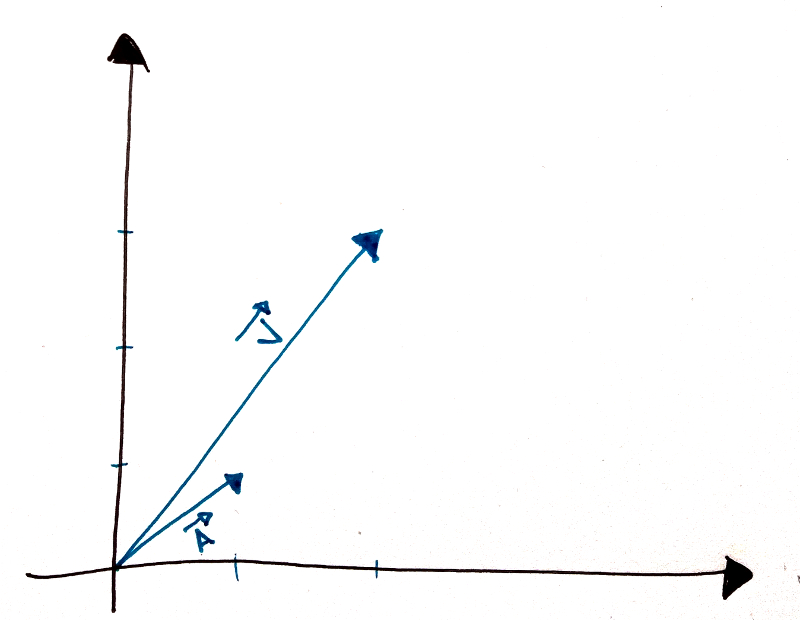
\includegraphics[width=0.4\textwidth]{./img/c4r1.jpg}
\end{figure}

A questão pede que decomponhamos $\overrightarrow{V}$ como soma de dois outros vetores. Vamos chamá-los de $\overrightarrow{V_A}$ e $\overrightarrow{V_B}$. Também é pedido que um deles, digamos $\overrightarrow{V_A}$, esteja na mesma direção de $\overrightarrow{A}$ enquanto que o outro, $\overrightarrow{V_B}$, seja perpendicular a ele.

Vamos focar em $\overrightarrow{V_A}$ por enquanto. Ele pode ser representado como mostrado abaixo.

\begin{figure}[h]
\centering
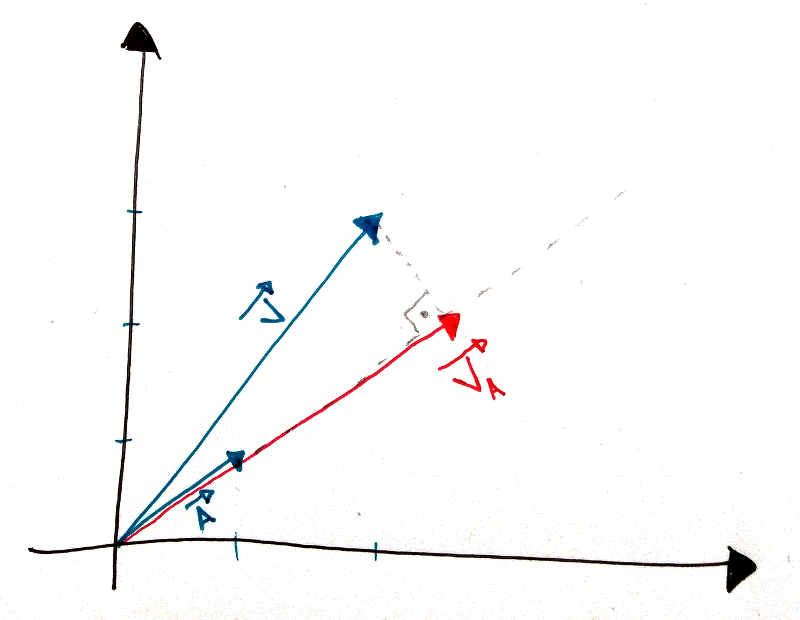
\includegraphics[width=0.4\textwidth]{./img/c4r2.jpg}
\end{figure}

Para obtê-lo, basta sabermos o comprimento da projeção ortogonal de $\overrightarrow{V}$ sobre $\overrightarrow{A}$ e então ajustarmos o comprimento de $\overrightarrow{A}$.

Como vimos em questões anteriores, o comprimento de $\overrightarrow{V_A}$ é obtido via cosseno do ângulo entre os vetores. O ângulo determinado por $\overrightarrow{A}$ é igual a 45\degree, pois suas duas dimensões são iguais. O cosseno do ângulo $\alpha$, determinado por $\overrightarrow{V}$, é igual a $\frac{1}{\sqrt{10}}=\frac{\sqrt{10}}{10} \approx 0,32$. Portanto, $\alpha = \arccos(0,32) \approx 71,6\degree$ e o ângulo entre os vetores é igual a $71,6-45=26,6$ graus.

Com base nessa informação, temos que o comprimento de $\overrightarrow{V_A}$ é dado por:

$$
\Arrowvert \overrightarrow{V_A} \Arrowvert = \cos(22,6) \cdot \sqrt{10} \approx 0,89 \cdot \sqrt{10}
$$

Agora, como $\overrightarrow{V_A}$ aponta para a mesma direção de $\overrightarrow{A}$, vamos fazer com que a norma de $\overrightarrow{A}$ seja igual ao valor que foi obtido acima.

Primeiro, dividimos as dimensões de $\overrightarrow{V_A}$ pela sua norma ($\sqrt{2}$): $(\frac{1}{\sqrt{2}};\frac{1}{\sqrt{2}})$.

Segundo, multiplicamos o resultado obtido acima pela norma desejada ($0,89 \cdot \sqrt{10}$): $(\frac{0,89 \cdot \sqrt{10}}{\sqrt{2}};\frac{0,89 \cdot \sqrt{10}}{\sqrt{2}}) = (0,89 \cdot \sqrt{5};0,89 \cdot \sqrt{5})$.

Esse é o vetor $\overrightarrow{V_A}$. Note que suas coordenadas podem ser approximadas para $(2,0;2,0)$.

A segunda parte da questão é mais simples. O enunciado nos pediu que o $\overrightarrow{V}$ seja decomposto como uma soma de dois vetores, ou seja, $\overrightarrow{V}=\overrightarrow{V_A}+\overrightarrow{V_B}$, como já obtivemos $\overrightarrow{V_A}$, temos que $\overrightarrow{V_B}=\overrightarrow{V}-\overrightarrow{V_A}$, logo: $\overrightarrow{V_B}=(1;3)-(2;2)=(-1;1)$.

Representando todos os vetores na figura abaixo, note que as dimensões de $\overrightarrow{V_B}$ são compatíveis com o que foi pedido pela questão, $\overrightarrow{V_A}$ e $\overrightarrow{V_B}$ serem perpendiculares, e eles são a resposta final.

\begin{figure}[h]
\centering
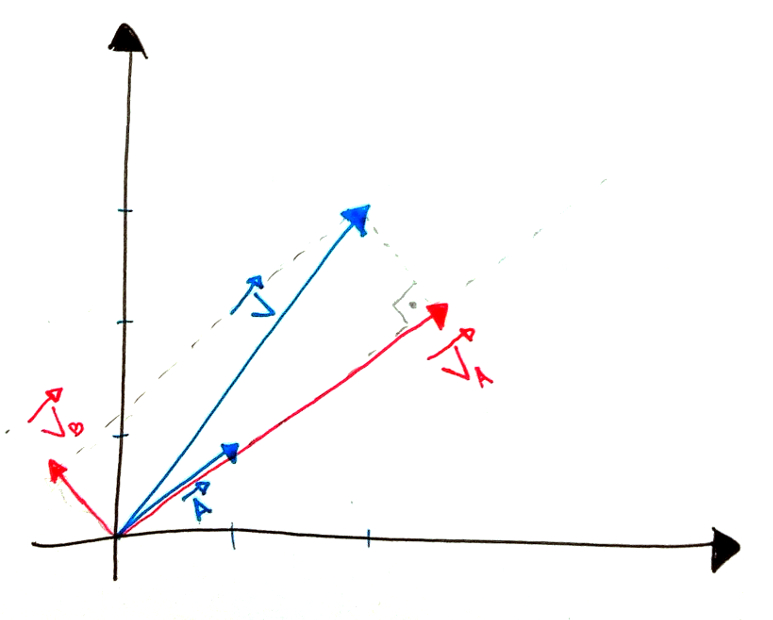
\includegraphics[width=0.4\textwidth]{./img/c4r3.jpg}
\end{figure}

Agora, tente aplicar o mesmo raciocínio para resolver a questão a seguir. Tente ser estratégico no uso de frações ou aproximações.

\begin{resolva}
Decomponha o vetor $\overrightarrow{V}=(3;4)$ como soma de dois vetores perpendiculares de modo que um deles esteja na mesma direção do vetor $\overrightarrow{A}=(12;5)$.
\end{resolva}

\newpage

\section{Gabarito}

\imprimeGabarito

\section{Registro de progresso}

Essa parte por enquanto fica com conteúdo vazio até que seja decidido como será feito o controle do progresso.
\vspace{5cm}

\section{Auto-avaliação final}
Avalie o quanto você acha que sabe sobre os seguintes itens após ter resolvido as questões deste capítulo.

\begin{center}
 \begin{tabular}{|p{35mm}||p{15mm}|p{15mm}|p{15mm}|p{15mm}|} 
 \hline
   & Nada & Muito pouco & Noções gerais & Bastante\\
 \hline
 Calcular seno e cosseno em um triângulo retângulo &  &  &  &  \\ 
 \hline
 Obter um ângulo sabendo o seu seno ou cosseno &  &  &  &  \\
 \hline
 Usar seno e cosseno em uma calculadora &  &  &  &  \\
 \hline
 Representar vetores &  &  &  &  \\
 \hline
\end{tabular}
\end{center}

Cheque como foi o seu progresso comparando essas respostas com as que você deu antes de estudar este capítulo. Caso você não tenha atingido o nível ``Bastante''  em algum dos tópicos acima, liste abaixo qual ação concreta você fará nos próximos dias para atingi-lo:

\vspace{0.3cm}

\noindent\rule{\linewidth}{0.4pt}

\noindent\rule{\linewidth}{0.4pt}

\noindent\rule{\linewidth}{0.4pt}

\end{document}
